\chapter{Literature Review} \label{chap:literatureReview}

%\version{v1.10.2015}

\section*{}
\section*{Carpooling}
\section{Definition and general principle}
Carpooling (also car-sharing, ride-sharing and lift-sharing) is the sharing of car journeys       so that more than one person travels in a car, and prevents the need for others to have to drive to a location themselves.
\\ By having more people using one vehicle, carpooling reduces each person's travel costs 
such as: fuel costs, tolls, and the stress of driving. Carpooling is also a more environmentally 
friendly and sustainable way to travel as sharing journeys reduces air pollution, carbon 
emissions, traffic congestion on the roads, and the need for parking spaces. Authorities 
often encourage carpooling, especially during periods of high pollution or high fuel prices.
Car sharing is a good way to use up the full seating capacity of a car, which would otherwise 
remain unused if it were just the driver using the car.
\\ In 2009, carpooling represented 43.5% of all trips in the United States and 10% of 
commute trips. The majority of carpool commutes (over 60%) are "fam-pools" with family 
members.
\\ Carpool commuting is more popular for people who work in places with more jobs 
nearby, and who live in places with higher residential densities. Carpooling is significantly 
correlated with transport operating costs, including fuel prices and commute length, and 
with measures of social capital, such as time spent with others, time spent eating and 
drinking and being unmarried. However, carpooling is significantly less likely among 
people who spend more time at work, elderly people, and homeowners. 
\\ Carpooling usually means to divide the travel expenses equally between all the 
occupants of the vehicle (driver or passenger). The driver does not try to earn money, but 
to share with several people the cost of a trip he would do anyway. The expenses to be 
divided basically include the fuel and possible tolls. But if we include in the calculation the 
depreciation of the vehicle purchase and maintenance, insurance and taxes paid by the 
driver, we get a cost around 100DA/km. There are platforms that facilitate carpooling by 
connecting people seeking respectively passengers and drivers. Usually there is a fare set 
up by the car driver and accepted by passengers because they get an agreement before trip 
start.

\section{Carpooling Types}
\subsection{Regular}
The car is often perceived as an extension of the personal space, the driver, alone in 
his vehicle is in a closed space; he is free to do what he likes: listen to the radio, sing, call 
with headsets ... Carpooling regularly is to share a dialogue, experiences, stories.
In the United States an intermediate concept has developed between carpooling and 
the public transport line: the Vanpool. These are minibuses chartered by an employer, a 
public authority or a private company and made available to a group of people who 
regularly make the same journey.

\subsection{Occasional}
This type of carpooling is mainly used for leisure or last minute departures. The 
linking is often done through websites or mobile applications, which can significantly 
reduce travel costs, but usually requires to carpool with one or more unknown.
This type of carpooling is mainly used for leisure or last minute departures. The 
linking is often done through websites or mobile applications, which can significantly 
reduce travel costs, but usually requires to carpool with one or more unknown.

\subsection{Eventual}
Participants in an event (music festival, sporting event, wedding, associative or 
institutional meeting ...) can organize to carpool to the venue of the event. This one-time 
carpool has a special feature: all participants travel to the same place on the same date.
Carpooling is also used for departures on holidays or weekends, savings on a trip 
being even larger than the trip is long. So carpooling becomes an alternative of affordable 
and accessible transportation.
\\ There are also "cultural" carpooling platforms to visit a cultural site: castles, 
museums, exhibitions, artists' studios, religious places, festivals, etc.
\section{Requirement Specification}
\subsection{Existing System for carpooling}
Many carpoolings applications and websites have been developed around the world. A similar carpooling system was developed in Massey University New Zealand by a group of students to allow students of Massey University, Albany campus to share their vehicle with non-vehicle owning students.
\\ Following some examples of carpooling systems around the globe : 
\subsection{Websites}
\begin{itemize}

\item New Zealand: https://www.asa.ac.nz/carpool
\item Algeria: www.nroho.com, www.m3aya.com,www.nsogo.net
\item Europe: BlaBlaCar.com, carpooling.com, GoMore.com
\item France: covoiturage.fr
\item USA: car.ma , www.rdvouz.com
\item World: Outpost.travel , joinntravel.com , www.letsride.in

\end{itemize}

\subsection{Mobile Applications}
\begin{itemize}

\item New Zealand: ASA
\item Algeria: YAssir,Nsogo, AMIR
\item World: Uber, sRide, RideShare, 
\item USA: Uber, Lyft
\item France: Karos, Wever, BlaBlaCar, OuiHop

\end{itemize}
\section{Proposed System}
Our purposed system is a “Carpool” application which is a ride sharing application designed just for students.students can login or signup to this application only via university email id to make sure that only enrolled students in a university used this application.
\\ Vehicle owning students can share their rides with other students for traveling to and from their institutes and earn money.

\section{Requirement Specifications}
It involves functional and non-functional functionalities that must be performed by the system:

\subsection{Functional Requirements}

\begin{figure}[h]
\subsubsection{Table 1: Functional Requirement - 01}
\centering
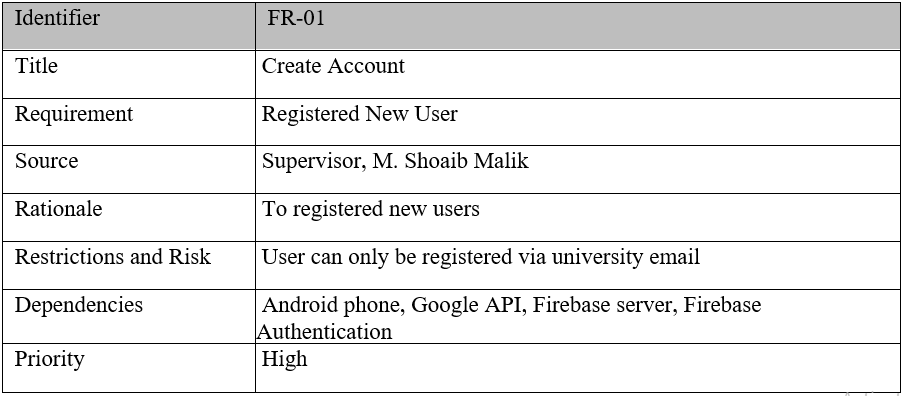
\includegraphics[width=0.8\textwidth]{TableFR1}
\end{figure}

\begin{figure}[h]
\subsubsection{Table 2: Functional Requirement - 02}
\centering
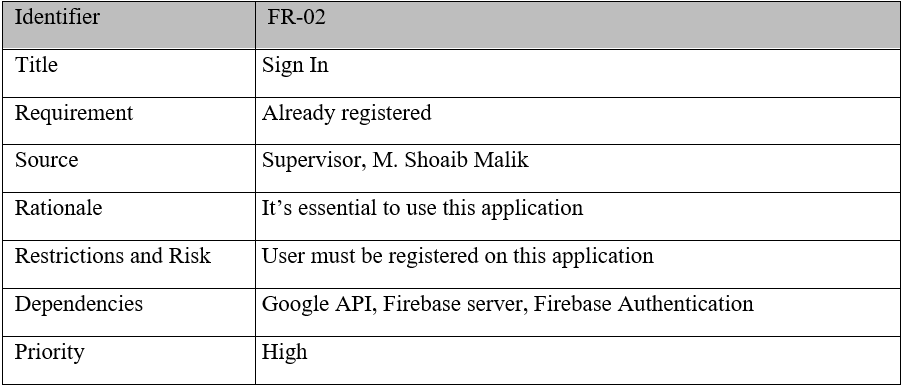
\includegraphics[width=0.8\textwidth]{TableFR2}
\end{figure}

\begin{figure}[h]
\subsubsection{Table 3: Functional Requirement - 03}
\centering
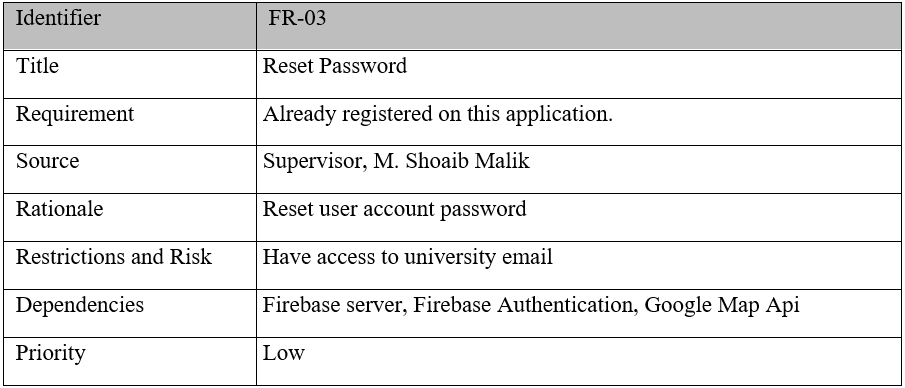
\includegraphics[width=0.8\textwidth]{TableFR3}
\end{figure}

\begin{figure}[h]
\subsubsection{Table 4: Functional Requirement - 04}
\centering
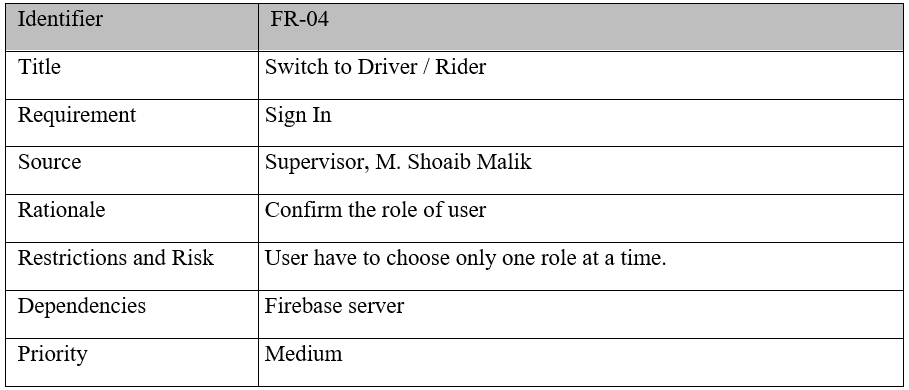
\includegraphics[width=0.8\textwidth]{TableFR4}
\end{figure}

\begin{figure}[h]
\subsubsection{Table 5: Functional Requirement - 05}
\centering
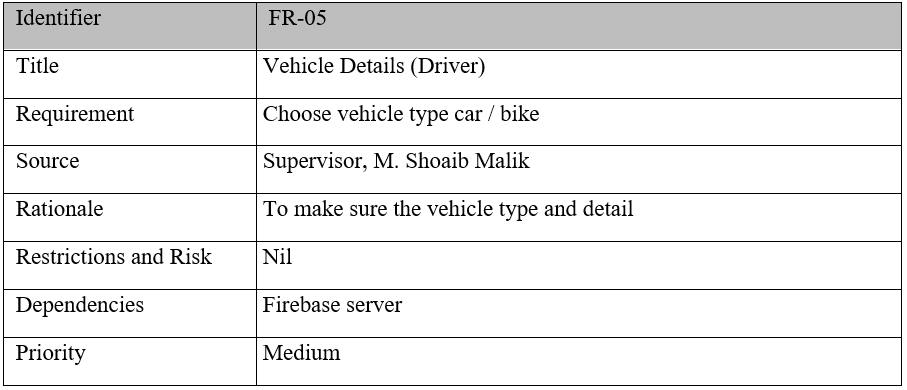
\includegraphics[width=0.8\textwidth]{TableFR5}
\end{figure}

\begin{figure}[h]
\subsubsection{Table 6: Functional Requirement - 06}
\centering
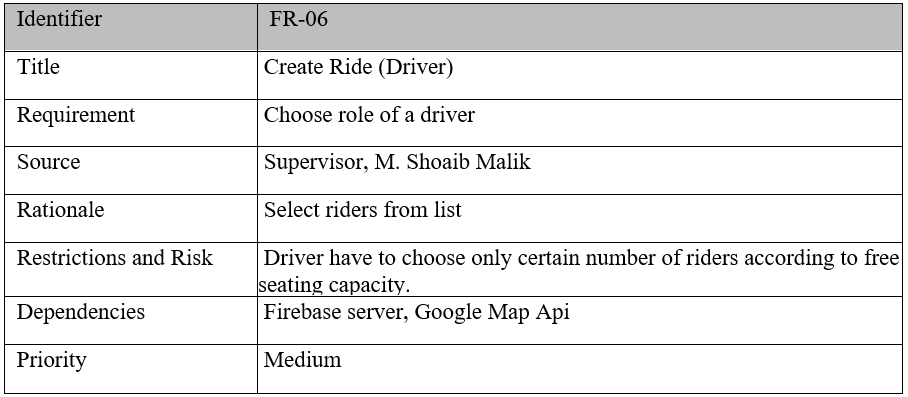
\includegraphics[width=0.8\textwidth]{TableFR6}
\end{figure}

\begin{figure}[h]
\subsubsection{Table 7: Functional Requirement - 07}
\centering
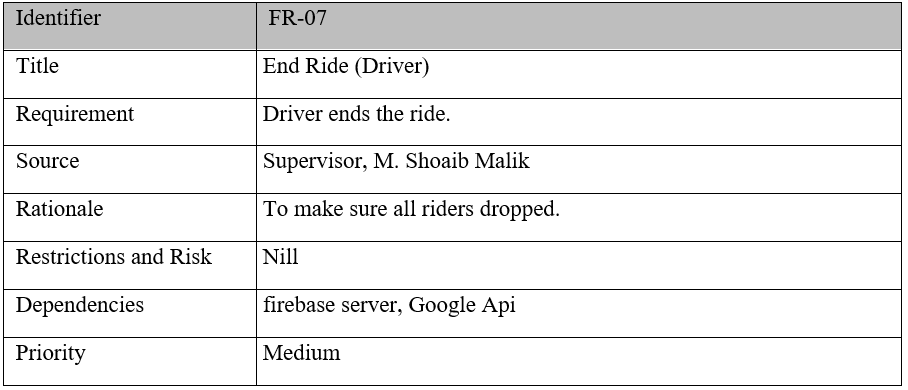
\includegraphics[width=0.8\textwidth]{TableFR7}
\end{figure}

\begin{figure}[h]
\subsubsection{Table 8: Functional Requirement - 08}
\centering
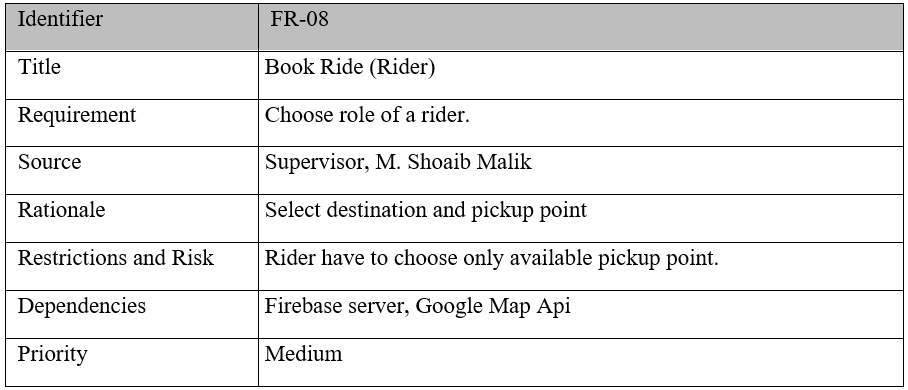
\includegraphics[width=0.8\textwidth]{TableFR8}
\end{figure}

\begin{figure}[h]
\subsubsection{Table 9: Functional Requirement - 09}
\centering
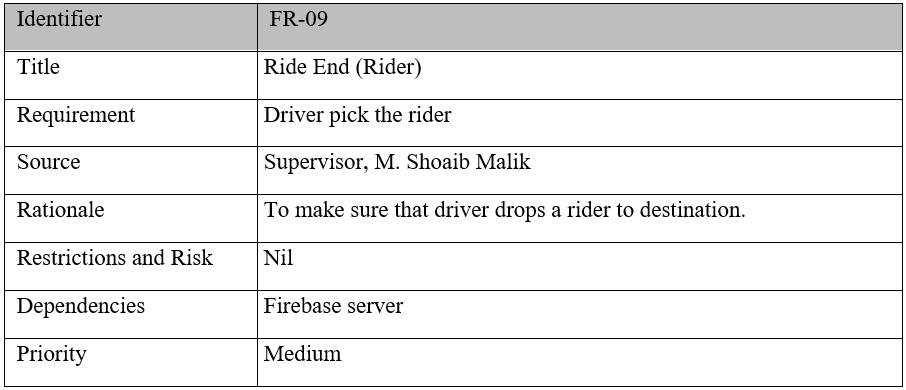
\includegraphics[width=0.8\textwidth]{TableFR9}
\end{figure}

\begin{figure}[h]
\subsection{Non-Functional Requirements} 
\bigskip
\bigskip
\subsubsection{Table 10: Non-Functional Requirement - 01}
\centering
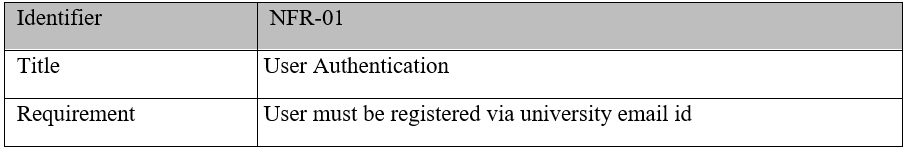
\includegraphics[width=0.8\textwidth]{TableNFR1}
\end{figure}

\begin{figure}[h]
\subsubsection{Table 11: Non-Functional Requirement - 02}
\centering
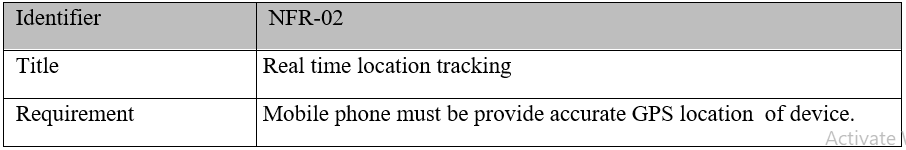
\includegraphics[width=0.8\textwidth]{TableNFR2}
\end{figure}

\begin{figure}[h]
\subsubsection{Table 12: Non-Functional Requirement - 03}
\centering
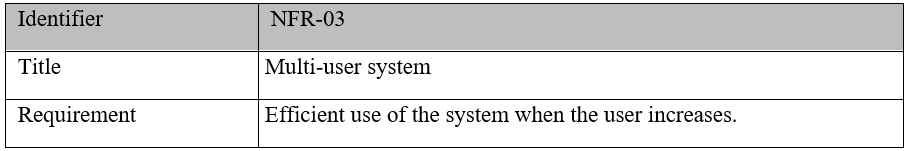
\includegraphics[width=0.8\textwidth]{TableNFR3}
\end{figure}

\begin{figure}[h]
\subsubsection{Table 13: Non-Functional Requirement - 04}
\centering
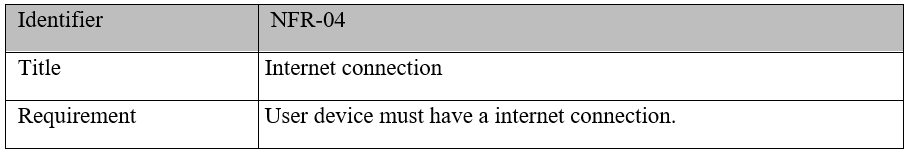
\includegraphics[width=0.8\textwidth]{TableNFR4}
\end{figure}

\begin{figure}[h]
\subsubsection{Table 14: Non-Functional Requirement - 05}
\centering
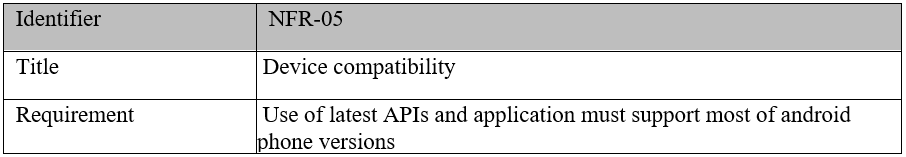
\includegraphics[width=0.8\textwidth]{TableNFR5}
\end{figure}

\begin{figure}[h]
\subsubsection{Table 15: Non-Functional Requirement - 06}
\centering
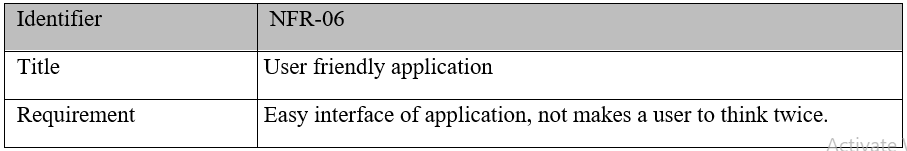
\includegraphics[width=0.8\textwidth]{TableNFR6}
\end{figure}

\begin{figure}[h]
\subsubsection{Table 16: Non-Functional Requirement - 07}
\centering
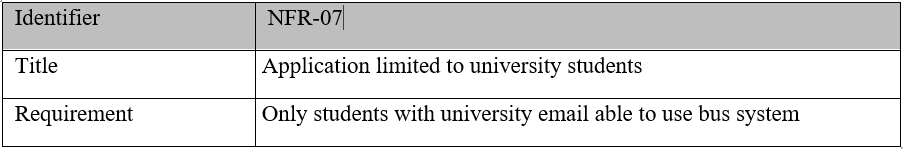
\includegraphics[width=0.8\textwidth]{TableNFR7}
\end{figure}

\begin{figure}
\section{Use Cases}
\subsection{Use Case Diagram}
\center
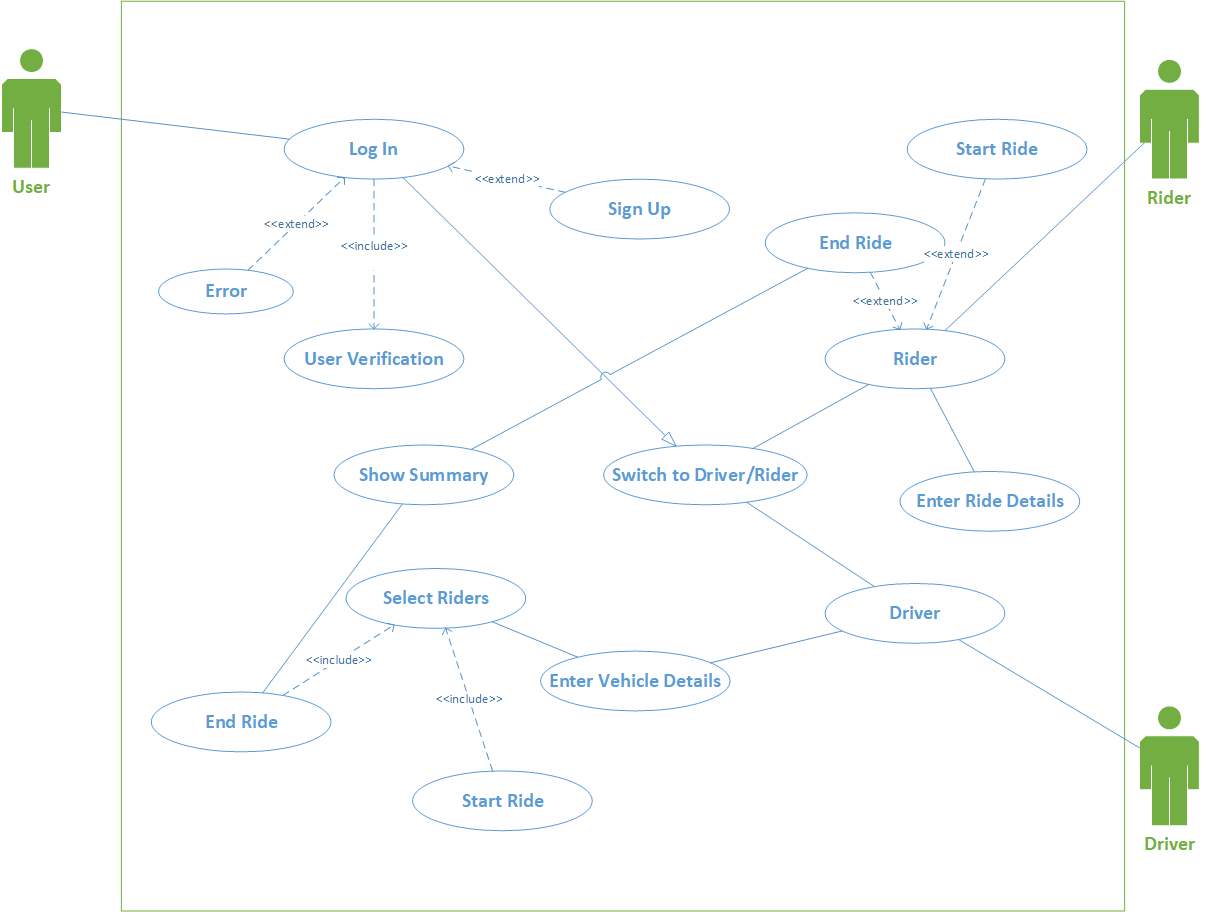
\includegraphics[width=1.2\textwidth]{UseCaseDiagram}
\caption{Use Case Diagram}
\label{fig:UseCaseDiagram}
\end{figure}